% !TeX spellcheck = en_GB

\section{\protect{\emoji{chipmunk}} \textit{Deep Learning} in a nutshell}{

    \begin{frame}{\protect{\emoji{chipmunk}} \textit{Deep Learning}: a definition}

        \begin{block}{\textit{Deep Learning}}
            \textit{Deep Learning} is (probabilistic) \alert{\textit{machine learning}} with \textit{deep artificial \alert{neural networks}, operating in (strongly) \alert{overparametrised} regime.}
        \end{block}
        \begin{center}
            OK, but what does it mean?
        \end{center}

    \end{frame}

    \begin{frame}{\protect{\emoji{chipmunk}} \textit{Deep Learning} $\subseteq$  \textit{Machine Learning}}

        \begin{block}{\textit{Machine Learning}}

            \begin{quote}{\textsc{T. Mitchell}, \textit{attributed} -- 1997}
                \hfill\break
                A computer program is said to learn from experience E w.r.t. to some class of tasks
                T and performance measure P, if its performance at tasks in T, as measured by P,
                improves with experience E.
            \end{quote}
        \end{block}

        Allowing effective decoupling of:
        \begin{itemize}
            \item \alert{\textit{model}} (in our case: \textit{artificial neural networks})
            \item \alert{\textit{learning algorithm}} (in our case: \textit{loss} function minimisation; approximate, iterative, gradient based\footnote{Not strictly necessary, though})
        \end{itemize}
    \end{frame}
    \setcounter{footnote}{0}

    \begin{frame}{\protect{\emoji{chipmunk}} An intermezzo: \textit{Supervised Classification}}

        \underline{Focus scenario for today: \textit{supervised learning}}.
        \hfill\break

        \textit{Input} space: $\mathbb{I} \sim \mathbb{R}^{d}$ -- \textit{What} needs to be classified, or their embedding;\\
        \textit{Output} space: $\mathbb{O}$ -- Set of classes to \alert{partition} $\mathbb{I}$ in (or \textit{e.g.} \textit{logits}, \etc).\\
        \hfill\break
        \textit{Training set}: $\{\mathbb{I}\times\mathbb{O}\} \supseteq \mathbb{T} = \{(\vec{x}_1, \xi_1), (\vec{x}_2, \xi_2), \ \dots,\ (\vec{x}_n, \xi_n)\}$ -- Known examples;
        \hfill\break
        A classifier $\mathcal{N}_{\vec{\theta}, \vec{h}}: \ \mathbb{I} \rightarrow \mathbb{O}$ dependent from  \alert{parameters}\footnote{And statistics of the data; \textit{computed} rather than \textit{learned} optimisation-wise} ($\vec{\theta}$) and \alert{hyperparameters} ($\vec{h}$);\\
        A \alert{\textit{loss function}}: $\mathcal{L} = \mathcal{L}(\mathcal{N}_{\vec{\theta}, \vec{h}}, \mathbb{T})$ encoding the \textit{goodness} of the model on $\mathbb{T}$.
        \hfill\break

        \begin{block}{Goal of \textit{training}}

            Find optimal $\vec{\theta}$, \textit{i.e.} $\vec{\theta^{\star}} \coloneq \argmin_{\vec{\theta}}(\mathcal{L}(\mathbb{T} | \vec{\theta}, \mathcal{N}_{\vec{\theta},\vec{h}}))$
        \end{block}

    \end{frame}
    \setcounter{footnote}{0}

    \begin{frame}{\protect{\emoji{chipmunk}} The model: from \textit{neurons} to \textit{neural networks}}

        Preliminarily, we consider the \textit{vector-scalar} map $\netw{N}_{\textit{1n}}\colon \mathbb{R}^{d}\rightarrow\mathbb{R}$ (\textit{McCulloch-Pitts neuron}): an \alert{affine} transformation followed by a \alert{nonlinear} application, \textit{i.e.:}
        $$ y = \netw{N}_{\textit{1n}}(\vec{x}) = \mathcal{A}(b + \vec{w}\cdot\vec{x}) $$
        with learnable parameters $\vec{\theta} = (\vec{w}, b)$.

        For a \textit{vector-vector} map $\netw{N}_{\textit{1n}}\colon \mathbb{R}^{d}\rightarrow\mathbb{R}^{m}$, we operate element-wise \wrt the output, defining a \textit{neuron layer}, \textit{i.e.}:
        $$ \vec{y} = L(\vec{x}) = \mathcal{A}(\vec{b} + \mat{W}\vec{x}) \fullstop $$

        Such transformations can be composed, for (\alert{arbitrary}\footnote{Usually in the \textit{function space density} sense -- more generally \textit{PAC-ly} -- given \textit{width/depth} and growing the other.}) increased expressive power, in a \textit{fully connected}, \textit{feedforward} artificial neural network:
        $$ \vec{y} = \netw{N}(\vec{x}) = L_n(L_{n-1}(\dots L_2(L_1(\vec{x})))) \fullstop$$

    \end{frame}
    \setcounter{footnote}{0}

    \begin{frame}{\protect{\emoji{chipmunk}}Learning $\vec{\theta^{\star}}$: \textit{SGD \& friends}}

        We are left with an \alert{optimisation} problem in the (potentially \textit{very high-dimensional}) space of $\vec{\theta}$, that is generally \alert{intractable}. We resort to an \textit{iterative}, \textit{first-order}, approximate optimisation scheme. \textit{E.g.} (\textit{gradient descent with momentum}):

        $$ \vec{\theta^{\prime}} \leftarrow \vec{\theta} - \lambda\alert{\vec{g_i}} + \alert{\mu\vec{m}}$$
        $$ \vec{m^{\prime}} \leftarrow \vec{\theta^{\prime}} - \vec{\theta}\fullstop$$

        Usually, \textit{minibatch-aggregation}\footnote{Often, \textit{gradient averaging} over disjoint subsets of training data} and further \alert{regularisation} (\textit{e.g.} penalisation at \textit{loss} or \textit{weight} level\footnote{Source of the \textit{proper} $L_2$ \textit{vs.} \textit{proper weight decay} divergence.}) is employed.
    \end{frame}

    \begin{frame}{\protect{\emoji{chipmunk}} That's \textit{not} all, folks!}

        That was just a \textit{sneak peek}, and there is much much more...
        \begin{itemize}
            \item Different architectural \alert{\textit{inductive biases}} (\textit{e.g. convolutional-, graph- NNs});
            \item More advanced optimisers (\textit{e.g. EMA-based -- à la Adam, nested, $>1^{\textit{st}}$-order});
            \item Other regularisation strategies, \textit{convergence/generalisation} aids (\textit{i.e.} \textit{BatchNorm}, \textit{dropout});
            \item Learning rate scheduling and hyperparameter tuning;
            \item \alert{Efficient} gradient computation (\textit{e.g.} via \textit{BackProp});
            \item \textit{AutoDiff} internals, \etc\dots
        \end{itemize}
    \hfill\break
    We showed just a \textit{bare minimum} to allow what follows (\textit{but if time allows...}).

    \end{frame}

    \begin{frame}{\protect{\emoji{thinking-face}} \textit{Is everything clear?}}

    \textit{Fast-forwarding} to-date, \textit{deep learning} is a remarkably powerful and mature paradigm, able to reach (super)human-level performance in selected \textit{regression}, \textit{classification}, data \textit{generation} and \textit{control} tasks.

    \center 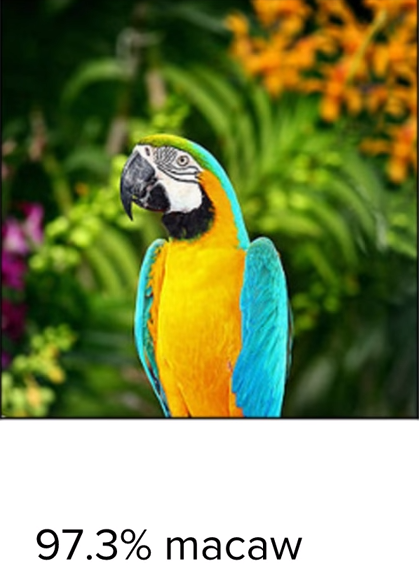
\includegraphics[height=0.35\linewidth]{macaw_macaw.png}
    \end{frame}

    \begin{frame}{\protect{\emoji{thinking-face}} \textit{Maybe not.}}

    \center 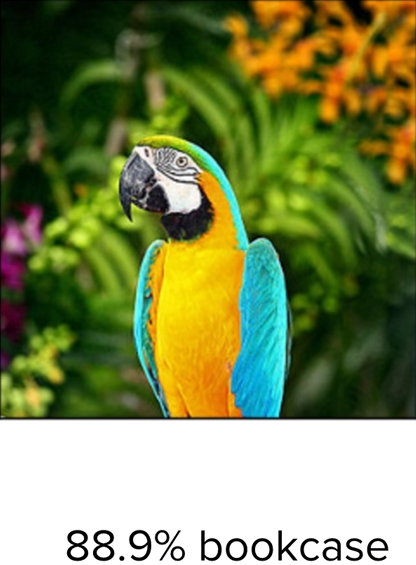
\includegraphics[height=0.35\linewidth]{macaw_bookcase.png}

    \hspace*{14px}\textit{(P. Perdikaris, 2018)}
    \end{frame}
    \setcounter{footnote}{0}
}